\chapter{Fixed Income Foundations}
\label{ch:fixed_income_foundations}
\chaptermark{Fixed income foundations}

This chapter fills the largest gap for a CS reader: the language of
\emph{fixed income} (bonds, interest rates, and swaps).
\Cref{ch:rates_derivatives,ch:credit_derivatives} depend on it.  Five
objects do all the work: zero rates $z(T)$, discount factors $D(T)$,
forward rates $f(T_1,T_2)$, duration $D_{\text{Mac}}$ (with convexity
$C$), and the par swap rate $s$.  No prior knowledge is assumed beyond
continuous discounting from \cref{ch:options_payoffs}.

\begin{backgroundbox}[Prerequisites]
From earlier in the book:
\begin{itemize}
  \item \Cref{ch:options_payoffs}: the risk-free rate $\rrf$,
    continuous discounting via $e^{-\rrf T}$, and the no-arbitrage
    principle.
  \item Basic calculus: derivatives of exponentials, Taylor expansion
    to second order.
\end{itemize}
\end{backgroundbox}


%% ================================================================
\section{Zero rates, discount factors, and forward rates}
\label{sec:fi_zero_forward}
%% ================================================================

Three objects underpin fixed income; every bond, swap, and rates
derivative is a function of them.

\subsection{Compounding conventions}

A rate $R$ per annum means different things depending on the
\emph{compounding frequency}~$m$:
\begin{itemize}
  \item \textbf{Annual} ($m=1$): \$1 grows to $(1+R)$ after one year.
  \item \textbf{Semi-annual} ($m=2$): \$1 grows to $(1+R/2)^2$ after
    one year.
  \item \textbf{Quarterly} ($m=4$): \$1 grows to $(1+R/4)^4$.
  \item \textbf{Continuous} ($m\to\infty$): \$1 grows to $e^R$.
\end{itemize}

In general, investing \$1 at a rate $R_m$ compounded $m$~times per
year for $n$~years gives a terminal value of
\begin{equation}
  V = \left(1 + \frac{R_m}{m}\right)^{mn}.
  \label{eq:discrete_compound}
\end{equation}
Taking $m \to \infty$ yields \emph{continuous compounding}:
\begin{equation}
  V = e^{R_c \, n},
  \label{eq:cont_compound}
\end{equation}
where $R_c$ is the continuously compounded rate.

\paragraph{Converting between conventions.}
Equating \cref{eq:discrete_compound,eq:cont_compound} at $n = 1$:
\begin{equation}
  e^{R_c} = \left(1 + \frac{R_m}{m}\right)^m
  \quad\Longrightarrow\quad
  R_c = m \ln\!\left(1 + \frac{R_m}{m}\right),
  \quad
  R_m = m\!\left(e^{R_c/m} - 1\right).
  \label{eq:rate_conversion}
\end{equation}

\begin{example}[Rate conversion]
10\% semi-annual ($m=2$) $\to$ continuous:
$R_c = 2\ln(1.05) = 9.758\%$.
8\% continuous $\to$ quarterly: $R_4 = 4(e^{0.02}-1) = 8.08\%$.
\end{example}

We use \textbf{continuously compounded rates} throughout unless stated
otherwise: rates over consecutive periods simply add
($e^{R_1 T_1} e^{R_2 T_2} = e^{R_1 T_1 + R_2 T_2}$), with no
re-compounding adjustments.

\subsection{Zero-coupon rates}

\begin{definition}[Zero-coupon rate (zero rate)]
\index{zero rate|textbf}\index{interest rate!zero rate|textbf}
\label{def:zero_rate}
The \emph{zero-coupon rate} (or simply \emph{zero rate}) $z(T)$ for
maturity $T$ is the annualised continuously compounded rate of return
earned on a riskless investment that pays no intermediate coupons,
made today and maturing at time $T$.  If you invest \$1 today at rate
$z(T)$, you receive $e^{z(T)\,T}$ at time~$T$.
\end{definition}

``Zero-coupon'' means no intermediate cash flows: a single lump sum
at maturity.  This is the purest interest rate: the price of
moving money from today to one future date.

The map $z : (0, \infty) \to \R$ is the \textbf{zero curve} (or
\textbf{term structure}).  It is typically upward-sloping: longer
maturities command higher rates.

\begin{pitfallbox}[Zero rates vs.\ coupon yields]
A zero rate is not a coupon-bond yield.  A 5-year 3\% Treasury's YTM
blends returns across many maturities (6m, 1y, \ldots, 5y); $z(5)$
is the return on a \emph{single} cash flow at year~5.  A YTM also
implicitly assumes every coupon is \emph{reinvested} at that same
YTM until maturity, an unrealistic assumption, since coupons paid
at year~1 will actually be reinvested at whatever the 1-year rate is
at that time.  Zero rates embed no reinvestment assumption: each
$z(T)$ is the clean price of moving money to one specific future
date.  The zero curve is the primitive; bond yields are derived
from it.
\end{pitfallbox}

\subsection{Discount factors}

\begin{definition}[Discount factor]
\index{discount factor|textbf}
\label{def:discount_factor}
The \emph{discount factor} $D(T)$ is the price today of a riskless
claim that pays exactly \$1 at time~$T$:
\begin{equation}
  D(T) \;=\; e^{-z(T)\,T}.
  \label{eq:discount_factor}
\end{equation}
\end{definition}

If $z(T) > 0$ then $D(T) < 1$.  To price a riskless cash-flow stream
$(c_i)$ at times $(t_i)$:
\begin{equation}
  \text{Price} \;=\; \sum_{i=1}^{n} c_i \, D(t_i).
  \label{eq:pv_cashflows}
\end{equation}
This is the \textbf{present-value identity}, the single most
important equation in fixed income.

\begin{intuitionbox}
$D(T)$ is the price today of \$1 at time~$T$.  $D(2) = 0.9139$ means
\$1 in two years is worth 91.39 cents today.
\end{intuitionbox}

Properties: $D(0) = 1$; $D$ strictly decreasing if rates positive;
$D(T) \to 0$ as $T \to \infty$; $D(T_1)/D(T_2)$ for $T_1 < T_2$ is
the discount factor for the forward period $[T_1, T_2]$.

\subsection{Forward rates}

Forward rates extend zero rates: the cost of lending between two
\emph{future} dates, implied by today's curve.  In plain English, the
forward rate $f(T_1,T_2)$ is the interest rate you can lock in
\emph{today} for a loan that will start at time $T_1$ and mature at
time $T_2$.  No money actually moves today, just a contractual
promise about the rate on a future loan.

\begin{definition}[Forward rate]
\index{forward rate|textbf}\index{interest rate!forward|textbf}
\label{def:forward_rate}
The \emph{(continuously compounded) forward rate} $f(T_1, T_2)$ for
the period from $T_1$ to $T_2$ (with $T_1 < T_2$) is the rate implied
by the zero curve such that lending from $T_1$ to $T_2$ is
consistent with lending from today to $T_1$ and from today to $T_2$.
\end{definition}

\paragraph{Derivation.}
Two strategies must give the same terminal value at $T_2$:
direct lending at $z(T_2)$ yields $e^{z(T_2)T_2}$; lending to $T_1$ at
$z(T_1)$ and rolling into a forward at $f(T_1,T_2)$ yields
$e^{z(T_1)T_1} e^{f(T_1,T_2)(T_2-T_1)}$.  By no-arbitrage:
\begin{equation}
  e^{z(T_1)\,T_1} \cdot e^{f(T_1,T_2)(T_2 - T_1)}
  \;=\; e^{z(T_2)\,T_2}.
  \label{eq:forward_no_arb}
\end{equation}
Taking logarithms and solving for $f$:
\begin{equation}
  \boxed{f(T_1, T_2)
    \;=\; \frac{z(T_2)\,T_2 - z(T_1)\,T_1}{T_2 - T_1}}\,.
  \label{eq:forward_rate}
\end{equation}

Equivalently, in terms of discount factors:
\begin{equation}
  \frac{D(T_1)}{D(T_2)}
  \;=\; e^{f(T_1,T_2)(T_2 - T_1)},
  \quad\text{so}\quad
  f(T_1,T_2) \;=\;
  \frac{\ln D(T_1) - \ln D(T_2)}{T_2 - T_1}.
  \label{eq:forward_from_D}
\end{equation}

\paragraph{Instantaneous forward rate.}
In the limit $T_2 \to T_1 = T$:
\begin{equation}
  f(T) \;\defeq\; \lim_{T_2 \to T} f(T, T_2)
  \;=\; z(T) + T\,z'(T)
  \;=\; -\frac{\partial}{\partial T}\ln D(T).
  \label{eq:instantaneous_forward}
\end{equation}
This is the \emph{instantaneous forward rate} at time~$T$: the
forward rate for an infinitesimally short period beginning at~$T$.

\begin{intuitionbox}
$f(T_1,T_2)$ is the break-even lending rate that makes an investor
indifferent between lending straight to $T_2$ at $z(T_2)$ or rolling
over from $T_1$.  It is \emph{not} a forecast but the rate
implied by today's curve.
\end{intuitionbox}

\paragraph{Upward-sloping curves and forward rates.}
\Cref{eq:forward_rate} can be rewritten as:
\begin{equation}
  f(T_1,T_2) = z(T_2) + (z(T_2) - z(T_1))\frac{T_1}{T_2 - T_1}.
  \label{eq:forward_above_zero}
\end{equation}
When the zero curve is upward-sloping ($z(T_2) > z(T_1)$), the
forward rate $f(T_1,T_2)$ exceeds the longer zero rate $z(T_2)$.
Conversely, when the curve is inverted, forward rates lie below the
zero curve.

\subsection{Worked example: computing $D$, $z$, and $f$}
\label{sec:fi_worked_zero}

Given $z(1) = 4\%$, $z(2) = 4.5\%$.

\paragraph{Step 1: Discount factors.}
\begin{align}
  D(1) &= e^{-0.04 \times 1} = 0.9608, \label{eq:D1_example}\\
  D(2) &= e^{-0.045 \times 2} = e^{-0.09} = 0.9139.
    \label{eq:D2_example}
\end{align}

\paragraph{Step 2: Forward rate.}
From \cref{eq:forward_rate}:
\begin{equation}
  f(1,2) = \frac{0.045 \times 2 - 0.04 \times 1}{2 - 1}
         = \frac{0.09 - 0.04}{1} = 5.00\%.
  \label{eq:f12_example}
\end{equation}

\paragraph{Step 3: Consistency check.}
$100 \times e^{0.04} \times e^{0.05} = 100 \times e^{0.09} =
100 \times e^{0.045 \times 2}$, matching 2-year lending at 4.5\%.
\checkmark

\paragraph{Full forward rate table.}
From the bootstrap example (\cref{sec:fi_bootstrap_example}):

\begin{center}
\begin{tabular}{ccc}
\toprule
\textbf{Year ($n$)} & \textbf{Zero rate $z(n)$ (\%)} &
  \textbf{1-year forward $f(n{-}1,n)$ (\%)} \\
\midrule
1 & 4.40 & --- \\
2 & 4.70 & $\frac{0.047 \times 2 - 0.044 \times 1}{1} = 5.00$ \\
3 & 4.83 & $\frac{0.0483 \times 3 - 0.047 \times 2}{1} = 5.09$ \\
4 & 4.96 & $\frac{0.0496 \times 4 - 0.0483 \times 3}{1} = 5.35$ \\
5 & 5.10 & $\frac{0.051 \times 5 - 0.0496 \times 4}{1} = 5.66$ \\
\bottomrule
\end{tabular}
\end{center}

Forward rates are the ``marginal'' rate, zero rates the ``average'':
the marginal exceeds the average exactly when the average is
rising (same relationship as marginal vs.\ average cost).

\paragraph{Interpreting forward rates.}
Forward rates are break-even rates, not forecasts.  The expectations
hypothesis equates them with expected future spot rates; empirically
they are biased upward by a \emph{term premium} compensating lenders
for longer-dated risk.  A steepening forward curve signals expected
rate rises or a rising term premium.

\paragraph{Visualising the zero and forward curves.}

\begin{center}
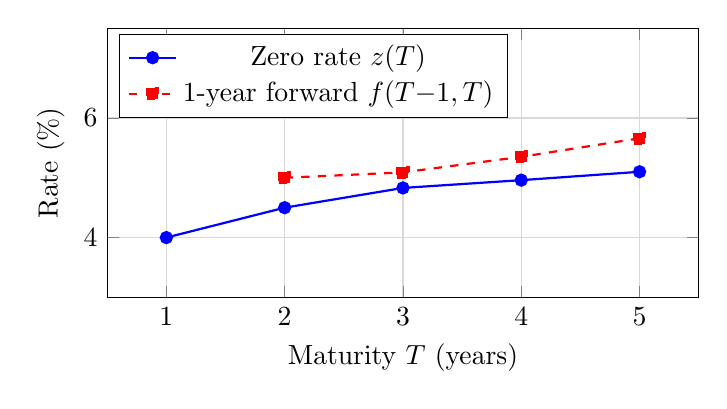
\begin{tikzpicture}
\begin{axis}[
  width=0.75\textwidth, height=5cm,
  xlabel={Maturity $T$ (years)},
  ylabel={Rate (\%)},
  xmin=0.5, xmax=5.5,
  ymin=3, ymax=7.5,
  legend style={at={(0.02,0.98)}, anchor=north west},
  grid=major, grid style={gray!30},
]
% Zero curve
\addplot[blue, thick, mark=*] coordinates {
  (1, 4.0) (2, 4.5) (3, 4.83) (4, 4.96) (5, 5.10)
};
\addlegendentry{Zero rate $z(T)$}
% Forward curve (1-year forward rates)
\addplot[red, thick, mark=square*, dashed] coordinates {
  (2, 5.0) (3, 5.09) (4, 5.35) (5, 5.66)
};
\addlegendentry{1-year forward $f(T{-}1,T)$}
\end{axis}
\end{tikzpicture}
\end{center}

On upward-sloping curves the forward curve lies above the zero curve
(\cref{eq:forward_above_zero}).

\begin{keyfactbox}[Zero rates and discount factors]
\begin{itemize}
  \item \textbf{Zero rate} $z(T)$: the annualised continuously
    compounded return for lending from today to time~$T$.
  \item \textbf{Discount factor} $D(T) = e^{-z(T)\,T}$: the price
    today of \$1 received at~$T$.
  \item \textbf{Forward rate}
    $f(T_1,T_2) = \frac{z(T_2)\,T_2 - z(T_1)\,T_1}{T_2 - T_1}$:
    the break-even rate for lending from $T_1$ to~$T_2$.
  \item These three are \emph{equivalent representations} of the
    same information: the \textbf{zero curve}
    $\{z(T) : T > 0\}$.
  \item When the zero curve slopes up, forward rates exceed zero
    rates.
\end{itemize}
\end{keyfactbox}


%% ================================================================
\section{Day-count conventions}
\label{sec:fi_daycount}
%% ================================================================

Rates are quoted annualised, but the cash flow depends on the accrual
days and the year definition.  A \textbf{day-count convention}
specifies both.

\begin{definition}[Day-count fraction]
\index{day-count convention|textbf}
The day-count fraction $\delta$ between dates $d_1,d_2$ is the
year-fraction under a specified convention.  The interest payment at
rate $R$ on notional $N$ is $N \times R \times \delta$.
\end{definition}

Three common conventions:

\paragraph{ACT/360.}
$\delta = (\text{actual days}) / 360$.  USD LIBOR, SOFR, Euribor, most
money-market instruments.  \emph{Ex.}~90-day period: $\delta = 0.2500$.
At 5\% on \$10\,M: \$125,000.

\paragraph{ACT/365 (Fixed).}
$\delta = (\text{actual days}) / 365$.  GBP SONIA, some AUD.
90-day period: $\delta = 0.2466$; \$10\,M at 5\%: \$123,288
(\$1,712 less than ACT/360).

\paragraph{30/360 (Bond Basis).}
30-day months, 360-day year:
\[
  \delta = \frac{360(Y_2-Y_1) + 30(M_2-M_1) + (D_2-D_1)}{360}.
\]
USD fixed-rate bond coupons and fixed legs of USD swaps.
Jan~15 to Apr~15: $\delta = 90/360 = 0.2500$.

\begin{pitfallbox}[Day-count matters for real money]
ACT/360 vs.\ ACT/365 on \$100\,M at 5\% for 90 days differs by
\$17,123.  Ignoring day-counts is a fast path to unexplained P\&L
breaks; every swap confirmation specifies the convention on each leg.
\end{pitfallbox}

The remainder of this chapter uses continuous compounding to avoid
day-count complications.  In practice, a Strat's first step when
building a pricer is getting day-counts right and unit-testing them.


%% ================================================================
\section{Bootstrapping the zero curve}
\label{sec:fi_bootstrap}
%% ================================================================

The market does not quote zero rates directly.  We observe prices of
deposits, futures, and swaps, and extract the implied rates, a
process called \textbf{bootstrapping}.  Start with the shortest-maturity instrument;
at each step use previously determined rates to solve for the next.

\subsection{The instruments}

A USD curve build uses three instrument types by maturity:

\begin{enumerate}
  \item \textbf{Deposits (0--6\,months).}  Interbank deposit rates are
    quoted as simple rates (no compounding).  A 3-month deposit at
    rate $r$ gives discount factor $D(T) = 1/(1+rT)$.

  \item \textbf{Futures (3\,months--2\,years).}  Eurodollar or SOFR
    futures are exchange-traded contracts on future short-term rates.
    Their prices directly imply forward rates, which can be converted
    to zero rates.  (We omit the convexity adjustment here; see
    \citeHull, Ch.~6.)

  \item \textbf{Swaps (2--30\,years).}  Par swap rates define the
    long end of the curve.  A par swap at rate~$s$ satisfies the
    par condition derived in \cref{sec:fi_par_swap}, which
    allows us to solve for the longest-maturity discount factor.
\end{enumerate}

\subsection{The bootstrap algorithm}

Sequentially:
\begin{enumerate}
  \item $D(T)$ from each deposit maturity.
  \item Extend using futures-implied forwards.
  \item For each swap maturity $T_k$ in increasing order, solve the
    par swap equation for $D(T_k)$ using previously determined $D$s.
\end{enumerate}

When intermediate $D$s are needed but undetermined (e.g.\ $D(3),D(4)$
for a 5-year swap), interpolate linearly in zero rates and solve
numerically.

\subsection{Five-point bootstrap: worked example}
\label{sec:fi_bootstrap_example}

We build a zero curve from five instruments:

\begin{center}
\begin{tabular}{llll}
\toprule
\textbf{\#} & \textbf{Instrument} & \textbf{Maturity} &
  \textbf{Rate} \\
\midrule
1 & 3-month deposit    & 0.25\,y & 4.00\% simple \\
2 & 6-month deposit    & 0.50\,y & 4.20\% simple \\
3 & 1-year swap        & 1.00\,y & 4.50\% annual fixed \\
4 & 2-year swap        & 2.00\,y & 4.80\% annual fixed \\
5 & 5-year swap        & 5.00\,y & 5.20\% annual fixed \\
\bottomrule
\end{tabular}
\end{center}

\paragraph{Step 1: 3-month deposit ($T = 0.25$).}
Deposit rates are simple (uncompounded).  Investing \$1 at 4.00\% for
3~months returns $1.01$:
\begin{equation}
  D(0.25) = \frac{1}{1 + 0.04 \times 0.25} = \frac{1}{1.01}
           = 0.9901.
\end{equation}
Converting to a continuously compounded zero rate:
\begin{equation}
  z(0.25) = \frac{-\ln(0.9901)}{0.25} = \frac{0.009950}{0.25}
           = 3.98\%.
\end{equation}

\paragraph{Step 2: 6-month deposit ($T = 0.50$).}
\begin{equation}
  D(0.50) = \frac{1}{1 + 0.042 \times 0.50} = \frac{1}{1.021}
           = 0.9794,
  \qquad
  z(0.50) = \frac{-\ln(0.9794)}{0.50} = 4.16\%.
\end{equation}

\paragraph{Step 3: 1-year swap ($T = 1.00$).}
The par condition (derived in \cref{sec:fi_par_swap}) for annual
coupon $s = 4.50\%$: fixed-leg PV plus notional repayment equals par:
\begin{equation}
  s \cdot D(1) + D(1) = 1
  \quad\Longrightarrow\quad
  D(1) = \frac{1}{1 + s} = \frac{1}{1.045} = 0.9569.
\end{equation}
Zero rate: $z(1) = -\ln(0.9569)/1 = 4.40\%$.

\paragraph{Step 4: 2-year swap ($T = 2.00$).}
$s = 4.80\%$ at years~1 and~2.  Par condition:
$s \cdot D(1) + (1+s) \cdot D(2) = 1$.  With $D(1) = 0.9569$:
\begin{align}
  D(2) &= \frac{1 - 0.048 \times 0.9569}{1.048}
        = \frac{1 - 0.04593}{1.048}
        = \frac{0.95407}{1.048}
        = 0.9104. \\
  z(2) &= -\ln(0.9104)/2 = 4.70\%.
\end{align}

\paragraph{Step 5: 5-year swap ($T = 5.00$).}
$s = 5.20\%$, annual payments at years 1--5.  Interpolate linearly
between $z(2)$ and the unknown $z(5)$:
\[
  z(T) = z(2) + \frac{z(5) - z(2)}{5 - 2}(T - 2),
  \quad 2 < T \leq 5,
\]
so $D(3),D(4),D(5)$ are all functions of $z(5)$.  Substituting into
\begin{equation}
  0.052 \times [D(1) + D(2) + D(3) + D(4) + D(5)] + D(5) = 1
  \label{eq:bootstrap_5y}
\end{equation}
and solving numerically gives $z(5) = 5.10\%$.  Back-substituting:

\begin{center}
\begin{tabular}{ccc}
\toprule
\textbf{Maturity $T$} & \textbf{Zero rate $z(T)$} &
  \textbf{Discount factor $D(T)$} \\
\midrule
0.25 & 3.98\% & 0.9901 \\
0.50 & 4.16\% & 0.9794 \\
1.00 & 4.40\% & 0.9569 \\
2.00 & 4.70\% & 0.9104 \\
3.00 & 4.83\% & 0.8651 \\
4.00 & 4.96\% & 0.8199 \\
5.00 & 5.10\% & 0.7750 \\
\bottomrule
\end{tabular}
\end{center}

\paragraph{Verification.}
Annuity $A = \sum_{n=1}^{5} D(n) = 4.3273$; then
$sA + D(5) = 0.052 \times 4.3273 + 0.7750 = 1.0000$.  \checkmark

\begin{keyfactbox}[Bootstrapping the zero curve]
The zero curve is not directly observable.  It is \emph{bootstrapped}
from traded instruments:
\begin{enumerate}
  \item \textbf{Short end} ($\leq 6$\,months): deposit rates give
    discount factors directly via
    $D = 1/(1+rT)$.
  \item \textbf{Middle} (6\,months--2\,years): Eurodollar/SOFR
    futures.
  \item \textbf{Long end} ($\geq 2$\,years): par swap rates, solved
    sequentially using previously determined discount factors.
\end{enumerate}
Between bootstrapped points, zero rates are typically interpolated
linearly (or with cubic splines for smoother hedges).
\end{keyfactbox}

\subsection{Reference implementation}

The following Python function bootstraps a zero curve from deposit
rates and annual par swap rates.

\begin{lstlisting}[caption={Zero-curve bootstrap from deposits and annual swaps.},
  label={lst:bootstrap}]
import math

def bootstrap(deposits, swaps):
    """Bootstrap a zero curve.
    deposits: list of (T, simple_rate)
    swaps:    list of (T, par_rate), annual fixed
    Returns dict {T: (z, D)}."""
    curve = {}
    for T, r in deposits:
        D = 1.0 / (1 + r * T)
        z = -math.log(D) / T
        curve[T] = (z, D)

    for T_swap, s in sorted(swaps):
        known_sum = sum(
            s * curve[t][1]
            for t in sorted(curve) if t < T_swap)
        # D(T_swap) from par condition
        D = (1.0 - known_sum) / (1.0 + s)
        z = -math.log(D) / T_swap
        curve[T_swap] = (z, D)
    return curve
\end{lstlisting}


%% ================================================================
\section{Bonds: yield, duration, convexity, and DV01}
\label{sec:fi_bonds}
%% ================================================================

A \textbf{bond} promises fixed coupons and return of face value $F$
at maturity.  Understanding price sensitivity to rates is the core
skill of a rates trader.

\subsection{Bond pricing from the zero curve}

\begin{definition}[Bond price]
\index{bond!price|textbf}
A bond with face value $F$, coupon rate $c$ paid $m$~times per year,
and maturity~$T$ generates cash flows
$c_i = Fc/m$ at times $t_i = i/m$ for $i = 1, \ldots, mT - 1$,
and a final cash flow of $Fc/m + F$ at $t_{mT} = T$.
Its price is the present value of these cash flows:
\begin{equation}
  P \;=\; \sum_{i=1}^{mT} c_i \, D(t_i).
  \label{eq:bond_price}
\end{equation}
\end{definition}

The price depends on the entire zero curve: each cash flow is
discounted at its own rate.  Market convention, however, quotes bonds
via a single number: the yield.

\subsection{Yield to maturity}

\begin{definition}[Yield to maturity]
\index{yield to maturity (YTM)|textbf}\index{YTM|textbf}
The \emph{yield to maturity} (YTM) of a bond is the single
continuously compounded rate $y$ such that discounting all cash flows
at $y$ reproduces the bond's market price:
\begin{equation}
  P \;=\; \sum_{i=1}^{n} c_i \, e^{-y\,t_i}.
  \label{eq:ytm}
\end{equation}
The yield must be found numerically (there is no closed-form solution
for coupon-bearing bonds), typically by Newton--Raphson or bisection.
\end{definition}

Yield is a summary statistic: convenient for quoting, lossy for risk.
Two bonds with the same yield can have very different sensitivities.

\paragraph{Price--yield relationship.}
$P$ falls as $y$ rises:
\begin{itemize}
  \item $y > c$: the bond trades at a \textbf{discount} ($P < F$).
    The coupon is below the market rate, so the bond is worth less
    than face value.
  \item $y < c$: the bond trades at a \textbf{premium} ($P > F$).
  \item $y = c$: the bond trades at \textbf{par} ($P = F$).
\end{itemize}

\subsection{Duration: first-order sensitivity}
\label{sec:fi_duration}

Duration quantifies how much the bond price moves when yields move.
It is the rates trader's core hedging unit: if you own a bond with
5-year duration and want to be rate-neutral, you short an offsetting
position (a futures contract, another bond, or a swap) whose
duration-weighted size matches, so that a parallel shift in rates
leaves your book's value unchanged.

\begin{definition}[Macaulay duration]
\index{Macaulay duration|textbf}\index{duration!Macaulay|textbf}
The \emph{Macaulay duration} of a bond is:
\begin{equation}
  D_{\text{Mac}} \;=\; \frac{1}{P}\sum_{i=1}^{n} t_i \, c_i \,
    e^{-y\,t_i}
  \;=\; -\frac{1}{P}\frac{dP}{dy}.
  \label{eq:duration}
\end{equation}
\end{definition}

\paragraph{Derivation.}
Differentiating \cref{eq:ytm} with respect to $y$:
\begin{equation}
  \frac{dP}{dy} = \sum_{i=1}^{n} (-t_i) \, c_i \, e^{-y\,t_i}
  = -\sum_{i=1}^{n} t_i \, c_i \, e^{-y\,t_i}.
  \label{eq:dPdy}
\end{equation}
Dividing both sides by $-P$:
\begin{equation}
  -\frac{1}{P}\frac{dP}{dy}
  = \frac{\sum_{i=1}^{n} t_i \, c_i \, e^{-y\,t_i}}{P}
  = D_{\text{Mac}}.
\end{equation}
This is a PV-weighted average of cash-flow times:
\begin{equation}
  w_i = \frac{c_i \, e^{-y\,t_i}}{P}, \qquad
  \sum_{i=1}^{n} w_i = 1, \qquad
  D_{\text{Mac}} = \sum_{i=1}^{n} t_i \, w_i.
\end{equation}

The key result is:
\begin{equation}
  \boxed{\frac{\Delta P}{P} \;\approx\; -D_{\text{Mac}}
    \cdot \Delta y}\,.
  \label{eq:duration_approx}
\end{equation}

\begin{intuitionbox}
A bond with duration 4.67 loses about 4.67\% per 100\,bp yield rise.
Duration is measured in years but acts as a sensitivity multiplier,
not a time.
\end{intuitionbox}

\paragraph{Properties of duration.}
\begin{itemize}
  \item A zero-coupon bond has duration exactly equal to its maturity.
  \item Adding coupons \emph{reduces} duration (you get cash back
    sooner).
  \item Higher yields reduce duration (distant cash flows are
    discounted more heavily, shifting weight towards earlier periods).
  \item Duration of a portfolio is the weighted average of the
    individual durations, weighted by market value.
\end{itemize}

\subsection{Convexity: second-order sensitivity}

For large yield moves, we need the second-order correction.

\begin{definition}[Convexity]
\index{convexity|textbf}
\begin{equation}
  C \;=\; \frac{1}{P}\frac{d^2 P}{dy^2}
  \;=\; \frac{1}{P}\sum_{i=1}^{n} t_i^2 \, c_i \, e^{-y\,t_i}.
  \label{eq:convexity}
\end{equation}
\end{definition}

The improved price-change approximation (Taylor expansion to second
order) is:
\begin{equation}
  \boxed{\frac{\Delta P}{P}
  \;\approx\; -D_{\text{Mac}} \cdot \Delta y
            + \tfrac{1}{2}\,C \cdot (\Delta y)^2}\,.
  \label{eq:duration_convexity}
\end{equation}

For plain vanilla bonds $C > 0$: price falls \emph{less} than
duration predicts on rate rises, and rises \emph{more} on rate falls.

\begin{center}
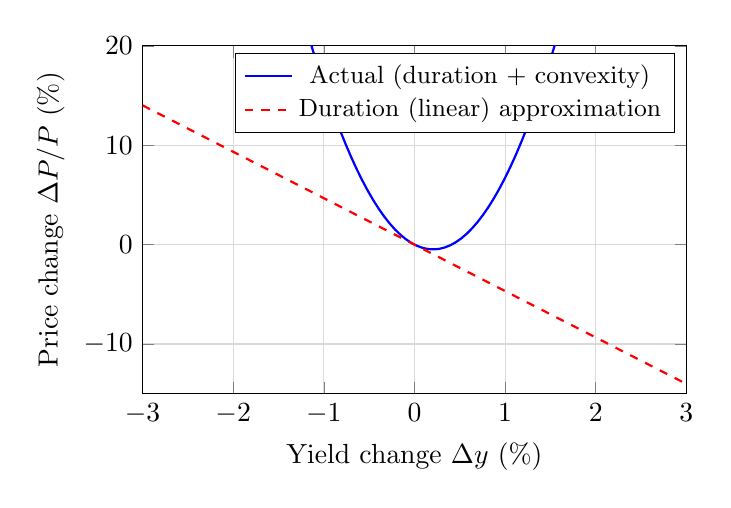
\begin{tikzpicture}
\begin{axis}[
  width=0.7\textwidth, height=6cm,
  xlabel={Yield change $\Delta y$ (\%)},
  ylabel={Price change $\Delta P / P$ (\%)},
  xmin=-3, xmax=3, ymin=-15, ymax=20,
  legend style={at={(0.98,0.98)}, anchor=north east, font=\small},
  grid=major, grid style={gray!30},
]
% True price-yield curve (convex)
\addplot[blue, thick, domain=-3:3, samples=100]
  {-4.67*x + 0.5*22.77*x*x/100*100};
\addlegendentry{Actual (duration + convexity)}
% Duration linear approx
\addplot[red, dashed, thick, domain=-3:3]
  {-4.67*x};
\addlegendentry{Duration (linear) approximation}
\end{axis}
\end{tikzpicture}
\end{center}

The blue curve is convexity in action; the red line (duration only)
overstates losses on rises and understates gains on falls.

\subsection{DV01: the risk metric}

\begin{definition}[DV01 (dollar value of one basis point)]
\index{DV01|textbf}\index{dollar value of one basis point|textbf}
\begin{equation}
  \text{DV01} \;=\; P \times D_{\text{Mac}} \times 0.0001.
  \label{eq:dv01}
\end{equation}
DV01 is the absolute dollar change in bond price per 1\,bp (0.01\%)
yield move, the standard rates-desk risk measure.  Portfolio DV01
sums across positions.
\end{definition}

\begin{intuitionbox}
Traders don't say ``duration 4.2''; they say ``long \$42,000 DV01.''
DV01 is the language of P\&L.
\end{intuitionbox}

\subsection{Worked example: 5-year 3\% semi-annual bond}
\label{sec:fi_bond_worked}

Consider a bond with face value $F = 100$, coupon rate 3\% paid
semi-annually (so each coupon is \$1.50), maturity $T = 5$~years,
and a continuously compounded yield of $y = 4\%$.

\paragraph{Step 1: Price.}
10 semi-annual periods: \$1.50 at $t = 0.5, \ldots, 4.5$ and \$101.50
at $t = 5.0$; discount at $e^{-0.04t}$.

\begin{center}
\small
\begin{tabular}{cccccc}
\toprule
$t$ (y) & CF (\$) & PV (\$) & Weight $w$ & $tw$ & $t^2 w$ \\
\midrule
0.5 &   1.50 &  1.4703 & 0.01542 & 0.00771 & 0.00386 \\
1.0 &   1.50 &  1.4412 & 0.01512 & 0.01512 & 0.01512 \\
1.5 &   1.50 &  1.4126 & 0.01482 & 0.02223 & 0.03334 \\
2.0 &   1.50 &  1.3847 & 0.01452 & 0.02905 & 0.05810 \\
2.5 &   1.50 &  1.3573 & 0.01424 & 0.03559 & 0.08898 \\
3.0 &   1.50 &  1.3304 & 0.01396 & 0.04187 & 0.12560 \\
3.5 &   1.50 &  1.3040 & 0.01368 & 0.04788 & 0.16757 \\
4.0 &   1.50 &  1.2782 & 0.01341 & 0.05363 & 0.21453 \\
4.5 &   1.50 &  1.2529 & 0.01314 & 0.05914 & 0.26613 \\
5.0 & 101.50 & 83.1012 & 0.87170 & 4.35848 & 21.79239 \\
\midrule
\multicolumn{2}{c}{\textbf{Total:}} & \textbf{95.3328} & 1.00000
  & \textbf{4.6707} & \textbf{22.7656} \\
\bottomrule
\end{tabular}
\end{center}

\paragraph{Step 2: Results.}
\begin{align}
  \text{Price} &= 95.33, \\
  D_{\text{Mac}} &= 4.6707 \text{ years}, \\
  C &= 22.7656, \\
  \text{DV01} &= 95.33 \times 4.6707 \times 0.0001
    = \$0.0445.
\end{align}

\paragraph{Step 3: Verification.}
If the yield rises by 1\,bp to $y = 4.01\%$, the exact new price
(re-summing all discounted cash flows) is $\$95.2883$, a change of
$-\$0.0445$.  Duration predicts
$\Delta P = -P \times D \times \Delta y = -95.33 \times 4.6707 \times
0.0001 = -\$0.0445$.  Exact match to four decimal places. \checkmark

For a larger move of $+100$\,bp ($y = 5\%$), duration alone predicts
$\Delta P = -\$4.45$, while the exact price is $\$91.07$, a drop of
$\$4.26$.  Including convexity:
\[
  \Delta P \approx -4.45 + \tfrac{1}{2}(95.33)(22.77)(0.01)^2
  = -4.45 + 0.11 = -\$4.34,
\]
much closer to the true answer.

\begin{keyfactbox}[Duration and DV01]
\begin{itemize}
  \item \textbf{Duration} $= -\frac{1}{P}\frac{dP}{dy}$: the
    percentage price sensitivity to yield changes.
  \item \textbf{DV01} $= P \times D \times 0.0001$: the dollar
    price change per 1\,bp yield move.
  \item Duration is a \emph{linear} approximation; \textbf{convexity}
    adds the curvature correction.
  \item A zero-coupon bond has duration equal to its maturity.
    Coupons reduce duration.
  \item \textbf{Risk is measured and hedged in DV01}, not in notional.
    A \$100\,M 30-year bond has far more DV01 than a \$100\,M 2-year
    bond.
\end{itemize}
\end{keyfactbox}

\subsection{Modified duration and dollar duration}
\label{sec:fi_modified_duration}

Macaulay duration assumes continuous compounding.  For yield quoted
with $m$ periods per year, differentiating
$P = \sum c_i (1 + y/m)^{-m t_i}$ gives:

\begin{definition}[Modified duration]
\index{modified duration|textbf}\index{duration!modified|textbf}
\begin{equation}
  D^* \;=\; \frac{D_{\text{Mac}}}{1 + y/m},
  \label{eq:modified_duration}
\end{equation}
where $m$ is the number of compounding periods per year.
The price-change approximation becomes $\Delta P \approx -P \cdot D^*
\cdot \Delta y$.
\end{definition}

Continuous compounding gives $D^* = D_{\text{Mac}}$; semi-annual
gives $D^*$ slightly smaller.

\paragraph{Dollar duration.}
$P \times D^*$ is the dollar price change per unit yield change;
DV01 $= $ dollar duration $/ 10{,}000$.

\subsection{Duration-based hedging}
\label{sec:fi_duration_hedge}

To immunise a bond portfolio against small parallel curve shifts,
construct a hedge so that total DV01 is zero.

\begin{example}[Hedging a bond with another bond]
\label{ex:duration_hedge}
You hold \$10\,M face value of a 10-year 5\% bond with modified
duration $D^*_A = 7.5$, priced at $P_A = 103$.  You want to hedge
using a 2-year 3\% bond with modified duration $D^*_B = 1.9$,
priced at $P_B = 99$.

Portfolio DV01:
$\text{DV01}_A = \$10{,}300{,}000 \times 7.5 \times 0.0001
= \$7{,}725$.

Required hedge face value $F_B$ satisfies:
\[
  F_B \times \frac{P_B}{100} \times D^*_B \times 0.0001
  = \$7{,}725,
\]
\[
  F_B = \frac{7{,}725}{0.99 \times 1.9 \times 0.0001}
  = \frac{7{,}725}{0.0001881}
  \approx \$41{,}069{,}644.
\]
Short approximately \$41.1\,M face of the 2-year bond to neutralise
DV01.  This protects against parallel shifts only, not curve
rotations; hence desks also monitor \emph{key rate DV01} (sensitivity
to individual curve points).
\end{example}

\begin{keyfactbox}[Duration-based hedging]
To hedge a bond position:
\begin{enumerate}
  \item Compute the DV01 of the position to be hedged.
  \item Choose a hedging instrument and compute its DV01 per unit.
  \item Determine the hedge ratio: $\text{Hedge notional} =
    \text{Position DV01} / \text{Hedge instrument DV01 per unit}$.
  \item \emph{Duration hedge protects against parallel shifts only.}
    For non-parallel (curve) risk, use multiple hedging instruments
    at different maturities.
\end{enumerate}
\end{keyfactbox}


%% ================================================================
\section{Repo}
\label{sec:fi_repo}
%% ================================================================

A \textbf{repurchase agreement} (\textbf{repo}) is a short-term
secured loan: the borrower sells a bond today and agrees to repurchase
it at a slightly higher price shortly.  The price difference is
interest at the \textbf{repo rate}.

\begin{definition}[Repo]
\index{repo|textbf}\index{repurchase agreement|textbf}
In a repo transaction, party~A (the borrower) sells securities to
party~B (the lender) at price~$P_0$ and agrees to repurchase them at
price $P_0(1 + r_{\text{repo}} \times \delta)$ after a period~$\delta$.
The collateral is the bond; the cash flow is the loan.
\end{definition}

\paragraph{Mechanics.}
\begin{center}
\begin{tikzpicture}[>=Stealth, node distance=4cm]
  \node[draw, rounded corners, minimum width=2.5cm,
    minimum height=1cm] (A) {Bond holder};
  \node[draw, rounded corners, minimum width=2.5cm,
    minimum height=1cm, right=5cm of A] (B) {Cash lender};
  \draw[->, thick, blue] (A.north east) -- node[above]{Bond}
    (B.north west);
  \draw[->, thick, red] (B.south west) -- node[below]{Cash $P_0$}
    (A.south east);
  \node[below=0.3cm of A, font=\small\itshape] {(borrower)};
  \node[below=0.3cm of B, font=\small\itshape] {(lender)};
  \node[above=0.8cm of $(A)!0.5!(B)$, font=\small]
    {Day 1: bond sold, cash received};
\end{tikzpicture}
\end{center}

At maturity the trade reverses: the borrower pays
$P_0(1 + r_{\text{repo}}\delta)$ and takes back the bond.

Key features:
\begin{itemize}
  \item The repo rate is the overnight secured lending rate, close to
    the central-bank policy rate (Fed Funds target in the US).
  \item \textbf{Overnight repo} renegotiates daily; \textbf{term repo}
    locks in a rate for a fixed period.
  \item Repo is how bond traders finance positions: repo bonds out
    overnight for cash, pay the repo rate (``leveraged book'').
  \item Spread between SOFR (unsecured) and repo reflects collateral
    quality: governments go at ``general collateral,'' others higher.
  \item A bond in demand for shorting repos below the general level;
    it is said to trade \emph{on special}.
\end{itemize}

\begin{intuitionbox}
Repo is a pawnshop for bonds: hand over collateral, receive cash, pay
interest.  The repo rate is the most fundamental short-term rate; SOFR
itself is computed from overnight Treasury repo.
\end{intuitionbox}


%% ================================================================
\section{Interest rate swaps}
\label{sec:fi_swaps}
%% ================================================================

The \textbf{interest rate swap} (IRS) is the most-traded derivative
in the world; 2024 notional outstanding exceeds \$500~trillion
\citeHull.

\subsection{What is an interest rate swap?}

\begin{definition}[Plain vanilla interest rate swap]
\index{interest rate swap (IRS)|textbf}\index{IRS|textbf}\index{swap!interest rate|textbf}
A \emph{plain vanilla interest rate swap} is an agreement between two
parties to exchange interest payments on a \emph{notional principal}
$N$ for a fixed number of years.  One party pays a \textbf{fixed rate}
$s$; the other pays a \textbf{floating rate} (typically SOFR, formerly
LIBOR).  The notional principal is never exchanged; it is used
only to calculate the interest payments.
\end{definition}

The two sides of the swap are called \textbf{legs}:
\begin{itemize}
  \item \textbf{Fixed leg}: pays $N \times s \times \delta$ at each
    payment date, where $\delta$ is the day-count fraction.
  \item \textbf{Floating leg}: pays $N \times r_{\text{float}} \times
    \delta$ at each payment date, where $r_{\text{float}}$ is the
    floating rate observed at the \emph{beginning} of the period.
\end{itemize}

Only the \emph{net} is exchanged: if fixed is \$2.60\,M and floating
\$2.40\,M, the fixed payer sends \$0.20\,M.

\paragraph{A picture of a swap.}
\begin{center}
\begin{tikzpicture}[>=Stealth, node distance=5cm]
  \node[draw, rounded corners, minimum width=3cm,
    minimum height=1.2cm, fill=blue!10] (A) {Party A};
  \node[draw, rounded corners, minimum width=3cm,
    minimum height=1.2cm, fill=red!10, right=5cm of A] (B) {Party B};
  \draw[->, thick, blue!70!black] ([yshift=3mm]A.east) --
    node[above, font=\small]{Fixed rate $s$}
    ([yshift=3mm]B.west);
  \draw[->, thick, red!70!black] ([yshift=-3mm]B.west) --
    node[below, font=\small]{Floating (SOFR)}
    ([yshift=-3mm]A.east);
  \node[below=0.5cm of A, font=\small\itshape]
    {``Fixed-rate payer''};
  \node[below=0.5cm of B, font=\small\itshape]
    {``Floating-rate payer''};
\end{tikzpicture}
\end{center}

\begin{example}[A 5-year IRS]
\label{ex:irs_basic}
Company~A enters a 5-year swap on \$100\,M notional:
\begin{itemize}
  \item A pays 5.13\% fixed, semi-annually.
  \item A receives 6-month SOFR, semi-annually.
\end{itemize}
Every six months, A pays $100\text{M} \times 0.0513 \times 0.5 =
\$2.57\text{M}$ fixed, and receives
$100\text{M} \times \text{SOFR}_{6m} \times 0.5$ floating.
If 6-month SOFR is 4.80\%, A receives \$2.40\,M and nets
$-\$0.17$\,M for that period.  If SOFR rises to 5.60\%, A receives
\$2.80\,M and nets $+\$0.23$\,M.
\end{example}

\subsection{Why swaps exist}

Three purposes:
\begin{enumerate}
  \item \textbf{Transform liabilities.}  A floating-rate borrower
    pays fixed in the swap to lock in borrowing costs.
  \item \textbf{Transform assets.}  A holder of fixed-rate bonds pays
    fixed / receives floating, converting the asset to floating-rate
    to match floating-rate liabilities.
  \item \textbf{Speculation.}  Expect rates to rise: pay fixed,
    receive floating; no bond purchase needed.
\end{enumerate}

\subsection{The par swap rate}
\label{sec:fi_par_swap}

A swap is worth zero at inception iff the fixed rate equals the
\textbf{par swap rate}.  We derive it from first principles.

\paragraph{Valuing the floating leg.}
A floating-rate bond resets to par at every payment date, since the
next coupon matches the market rate.  Hence:
\begin{equation}
  B_{\text{float}} = (N + k^*) \cdot D(t^*),
  \label{eq:float_bond}
\end{equation}
where $k^*$ is the next floating payment and $t^*$ the next payment
date.  At inception, $B_{\text{float}} = N$.  The PV of the floating
leg (netting the notional) is:
\begin{equation}
  \text{PV}_{\text{float}} = N - N \cdot D(T) = N\bigl(1 - D(T)\bigr).
  \label{eq:pv_float}
\end{equation}

\paragraph{Valuing the fixed leg.}
The fixed leg pays $N \cdot s \cdot \delta_i$ at each payment date
$t_i$.  Its present value is:
\begin{equation}
  \text{PV}_{\text{fixed}} = N \cdot s \sum_{i=1}^{n} \delta_i \,
    D(t_i).
  \label{eq:pv_fixed}
\end{equation}

\paragraph{Par condition.}
At inception, $\text{PV}_{\text{fixed}} = \text{PV}_{\text{float}}$:
\begin{equation}
  N \cdot s \sum_{i=1}^{n} \delta_i \, D(t_i) = N\bigl(1 - D(T)\bigr),
\end{equation}
and the par swap rate is:
\begin{equation}
  \boxed{s \;=\; \frac{1 - D(T)}{\displaystyle\sum_{i=1}^{n}
    \delta_i \, D(t_i)}}\,.
  \label{eq:par_swap_rate}
\end{equation}

The denominator $A = \sum \delta_i D(t_i)$ is the \textbf{annuity
factor} (or swap \textbf{PV01}): the PV of \$1 per annum on the
fixed-leg schedule.

\begin{keyfactbox}[IRS par swap rate]
The par swap rate is:
\[
  s = \frac{1 - D(T)}{\displaystyle\sum_{i=1}^{n} \delta_i\,D(t_i)}.
\]
\begin{itemize}
  \item Numerator $= 1 - D(T)$: the PV of the floating leg
    (net of notional).
  \item Denominator $= A$: the annuity factor, the PV of receiving
    \$1 per year on the fixed-leg payment schedule.
  \item The swap rate is completely determined by the zero curve.
\end{itemize}
\end{keyfactbox}

\begin{intuitionbox}
A swap is a portfolio of FRAs (each floating payment bets on one
forward rate).  The par swap rate is the single fixed rate making
the package worth zero; equivalently, it is the rate at which a
fixed bond exchanges for a floating bond, both at par.
\end{intuitionbox}

\subsection{Running example: 5-year IRS on \$100\,M}
\label{sec:fi_irs_example}

Using the bootstrapped curve from \cref{sec:fi_bootstrap}, price a
5-year semi-annual IRS on \$100\,M notional vs.\ 6-month SOFR.

\paragraph{Step 1: Discount factors.}
We need $D(t)$ at each semi-annual date; interpolate linearly in
zero rates where not directly bootstrapped:

\begin{center}
\begin{tabular}{cccc}
\toprule
$t$ (y) & $z(t)$ (\%) & $D(t)$ & Annuity contribution
  $0.5 \times D(t)$ \\
\midrule
0.5 & 4.16 & 0.9794 & 0.4897 \\
1.0 & 4.40 & 0.9569 & 0.4785 \\
1.5 & 4.55 & 0.9340 & 0.4670 \\
2.0 & 4.70 & 0.9104 & 0.4552 \\
2.5 & 4.83 & 0.8878 & 0.4439 \\
3.0 & 4.83 & 0.8651 & 0.4326 \\
3.5 & 4.96 & 0.8425 & 0.4213 \\
4.0 & 4.96 & 0.8199 & 0.4100 \\
4.5 & 5.10 & 0.7974 & 0.3987 \\
5.0 & 5.10 & 0.7750 & 0.3875 \\
\midrule
\multicolumn{3}{r}{\textbf{Annuity $A =$}} & \textbf{4.3842} \\
\bottomrule
\end{tabular}
\end{center}

\paragraph{Step 2: Par swap rate.}
\begin{equation}
  s = \frac{1 - D(5)}{A}
    = \frac{1 - 0.7750}{4.3842}
    = \frac{0.2250}{4.3842}
    = 5.13\%.
  \label{eq:par_rate_example}
\end{equation}

\paragraph{Step 3: Fixed payment.}
At the par rate of 5.13\%, the fixed payment every six months is:
\[
  N \times s \times \delta
  = \$100{,}000{,}000 \times 0.0513 \times 0.5 = \$2{,}566{,}254.
\]

\paragraph{Step 4: Verification.}
PV of fixed leg:
$N \times s \times A = \$100\text{M} \times 0.0513 \times 4.3842 =
\$22{,}502{,}042$.

PV of floating leg:
$N \times (1 - D(5)) = \$100\text{M} \times 0.2250 =
\$22{,}502{,}042$.

Swap value at inception: $\$0$.  \checkmark

\paragraph{Swap value after rates move.}
If the curve shifts up by 50\,bp, the floating leg is worth more; the
fixed leg's contractual rate is unchanged.  The fixed-rate payer
profits: they locked 5.13\% when the market now demands 5.63\%.
For a 1\,bp shift the swap value changes by
$N \times A \times 0.0001 = \$43{,}842$, the swap's DV01.

\subsection{Swap valuation after inception}

Once rates move, a traded swap acquires non-zero value.  From the
fixed-rate payer's perspective:
\begin{equation}
  V_{\text{swap}} = \text{PV}_{\text{float}} -
    \text{PV}_{\text{fixed}}
  = N(1 - D(T)) - N \cdot s_0 \cdot A_{\text{new}},
  \label{eq:swap_mtm}
\end{equation}
where $s_0$ is the original fixed rate and $A_{\text{new}}$ is the
annuity factor computed with today's (new) zero curve.

Equivalently, $V_{\text{swap}}$ equals the change in par rate times
the annuity:
\begin{equation}
  V_{\text{swap}} = N \cdot (s_{\text{current}} - s_0) \cdot
    A_{\text{new}}.
  \label{eq:swap_mtm_par}
\end{equation}
If par rates have risen above your locked-in rate, your swap (as
fixed-rate payer) is in the money.


%% ================================================================
\section{Yield curve shapes and term-structure theories}
\label{sec:fi_term_structure}
%% ================================================================

Understanding why the zero curve takes a particular shape is key to
reading market conditions.

\subsection{Four canonical curve shapes}

\begin{center}
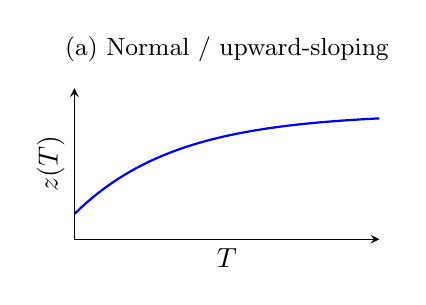
\begin{tikzpicture}
\begin{axis}[
  width=0.45\textwidth, height=3.5cm,
  title={\small (a) Normal / upward-sloping},
  xlabel={$T$}, ylabel={$z(T)$},
  xmin=0, xmax=10, ymin=0, ymax=6,
  axis lines=left, ticks=none,
]
\addplot[blue, thick, domain=0:10, samples=50]{5 - 4*exp(-0.3*x)};
\end{axis}
\end{tikzpicture}
\hfill
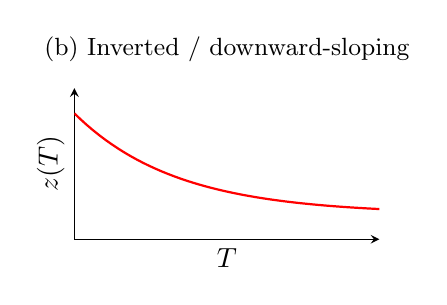
\begin{tikzpicture}
\begin{axis}[
  width=0.45\textwidth, height=3.5cm,
  title={\small (b) Inverted / downward-sloping},
  xlabel={$T$}, ylabel={$z(T)$},
  xmin=0, xmax=10, ymin=0, ymax=6,
  axis lines=left, ticks=none,
]
\addplot[red, thick, domain=0:10, samples=50]{1 + 4*exp(-0.3*x)};
\end{axis}
\end{tikzpicture}

\medskip

\begin{tikzpicture}
\begin{axis}[
  width=0.45\textwidth, height=3.5cm,
  title={\small (c) Flat},
  xlabel={$T$}, ylabel={$z(T)$},
  xmin=0, xmax=10, ymin=0, ymax=6,
  axis lines=left, ticks=none,
]
\addplot[black, thick, domain=0:10]{3.5};
\end{axis}
\end{tikzpicture}
\hfill
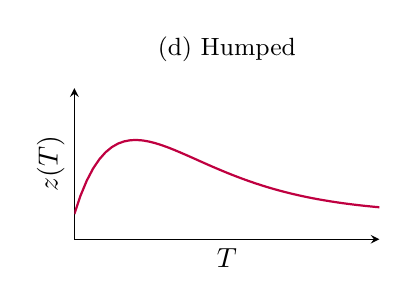
\begin{tikzpicture}
\begin{axis}[
  width=0.45\textwidth, height=3.5cm,
  title={\small (d) Humped},
  xlabel={$T$}, ylabel={$z(T)$},
  xmin=0, xmax=10, ymin=0, ymax=6,
  axis lines=left, ticks=none,
]
\addplot[purple, thick, domain=0:10, samples=50]
  {1 + 4*x*exp(-0.5*x)};
\end{axis}
\end{tikzpicture}
\end{center}

\begin{itemize}
  \item \textbf{Normal (upward-sloping):} most common; reflects the
    term premium for longer-horizon capital commitment.
  \item \textbf{Inverted:} short exceeds long; often a recession
    signal (market expects future cuts).  Every US recession since
    1960 was preceded by a 2s10s inversion.
  \item \textbf{Flat:} all maturities equal; transitional.
  \item \textbf{Humped:} rises then falls, reflecting near-term
    hikes and later cuts.
\end{itemize}

\subsection{Three theories of the term structure}

\paragraph{Expectations hypothesis.}
$z(T) = \frac{1}{T}\int_0^T \E[r(t)]\,dt$; forwards are unbiased
forecasts.  Empirically forwards overpredict spots, suggesting a
term premium.

\paragraph{Liquidity preference.}
Investors prefer short-term (more liquid, less price risk); borrowers
must offer a maturity-increasing liquidity premium.  Explains why the
curve is usually upward-sloping even when flat rates are expected.

\paragraph{Market segmentation.}
Institutional investors have preferred maturity habitats; curve shape
reflects segment-by-segment supply and demand.  Explains, e.g.,
persistent pension-fund demand for 30-year bonds.

Traders take the curve as given (bootstrapped) and hedge without
committing to a theory.  The theories matter for research
commentary, not pricing.


%% ================================================================
\section{OIS, basis swaps, and the LIBOR to SOFR transition}
\label{sec:fi_ois_sofr}
%% ================================================================

\subsection{Overnight indexed swaps (OIS)}

An \textbf{overnight indexed swap} (OIS) floats on the geometric
average of daily overnight rates rather than a term rate like 3-month
LIBOR.  Overnight references: effective fed funds (pre-2020) or SOFR
(post-2020) in the US; SONIA (UK); \texteuro STR (Eurozone).

\paragraph{Why OIS matters.}
\begin{itemize}
  \item Nearly risk-free (overnight, essentially secured).
  \item The \textbf{LIBOR--OIS spread} (3m LIBOR minus 3m OIS) is a
    stress indicator: $\sim$10\,bp normal, 364\,bp at the peak of the
    2007--09 crisis.
  \item Post-2020, clearinghouses discount using OIS curves (SOFR OIS
    in the US), not LIBOR.
\end{itemize}

\subsection{Basis swaps}

A \textbf{basis swap} has both legs floating against different rates
(e.g.\ 3m SOFR vs.\ 6m SOFR, or SOFR vs.\ fed funds).  The gap is
the \textbf{basis spread}.  Participants use them to manage benchmark
mismatches between assets and liabilities.

\subsection{The LIBOR to SOFR transition}

LIBOR (London Interbank Offered Rate) underpinned \$300+ trillion of
contracts: it was the floating rate in most swaps, loans, and rates
derivatives.

\paragraph{Why LIBOR was retired (30 June 2023).}
\begin{enumerate}
  \item \textbf{Manipulation scandal (2012).}  Traders manipulated
    submissions; Barclays, UBS, Deutsche Bank and others paid
    billions in fines.
  \item \textbf{Structural decline.}  The interbank market LIBOR
    measured had shrunk to near-zero volume; submissions became
    ``expert judgment,'' not transactions.
\end{enumerate}

\paragraph{SOFR as replacement.}
The Secured Overnight Financing Rate, administered by the NY Fed, is
based on overnight Treasury repo (\$1\,T+ daily volume), far more
robust than LIBOR.

Key differences from LIBOR:
\begin{itemize}
  \item LIBOR was forward-looking \emph{term} (3m LIBOR set at the
    start of the 3-month period); SOFR is backward-looking
    \emph{overnight} (compound daily observations ``in arrears'' to
    get a term rate).
  \item SOFR is \emph{secured} (repo); LIBOR was unsecured.  SOFR is
    systematically lower.
  \item Transition required amending trillions in legacy contracts.
\end{itemize}

\begin{pitfallbox}[SOFR is not a drop-in replacement for LIBOR]
Because SOFR is overnight and secured while LIBOR was term and
unsecured, simply replacing ``LIBOR'' with ``SOFR'' in a contract
changes its economics.  The ISDA fallback protocol adds a credit
spread adjustment (typically 26\,bp for 3-month tenor) to SOFR when
replacing LIBOR in legacy contracts.  Getting this adjustment wrong
creates P\&L breaks.
\end{pitfallbox}


%% ================================================================
%% Prosperity, GS, and History boxes
%% ================================================================

\begin{prosperitybox}
Prosperity lacks fixed-income products, but $D(T)$ is universal: any
cross-period strategy comparison uses $\text{PV} = \sum c_i D(t_i)$.
Build a simple discount curve from the round parameters as step one
in multi-period problems.  Forward rates show up implicitly in
lock-in-now-or-wait decisions: the forward is the break-even rate.
\end{prosperitybox}

\begin{gsbox}
A GS rates desk rebuilds the zero curve every morning from deposit
rates, futures, and swap quotes.  The ``morning curve build'' is the
Strat's critical daily deliverable: every swap, bond, swaption,
cap, floor, and structured product reprices off it.  Wrong curve
$\Rightarrow$ wrong prices and wrong hedge ratios desk-wide.

The Strat owns the curve code (usually SecDB/Slang), interpolation
choice (linear-in-zeros simple, cubic spline or monotone convex
fancier), and the bootstrap instrument set.  Traders flag the curve
in real time when it looks off, typically because a new instrument
is trading or an existing one has gone stale.

A junior Strat's first project is often to improve the build: add an
instrument, fix a day-count bug, or switch interpolation method.
Such projects are excellent because they touch the whole rates
infrastructure.
\end{gsbox}

\begin{historybox}
The first IRS was a 1981 IBM/World Bank deal arranged by Salomon
Brothers: IBM had DM and CHF bonds it wanted synthetically converted
to dollars; the World Bank wanted DM/CHF but borrowed cheaper in
dollars.  From there the market grew explosively: \$1\,T by 1987,
\$60\,T by 2000, \$500\,T+ by 2024, making swaps the largest
derivatives market in the world (larger than any single country's
government bond market).
\end{historybox}


%% ================================================================
\section*{Key facts to memorise}
\label{sec:fi_key_facts}
%% ================================================================

\begin{enumerate}
  \item \textbf{Zero rate} $z(T)$: continuously compounded rate for
    lending from now to~$T$.

  \item \textbf{Discount factor}: $D(T) = e^{-z(T)\,T}$, the
    price today of \$1 at~$T$.

  \item \textbf{Forward rate}:
    $f(T_1,T_2) = \frac{z(T_2)T_2 - z(T_1)T_1}{T_2 - T_1}$.
    Forward rates exceed zero rates when the curve slopes up.

  \item To convert between compounding conventions:
    $R_c = m\ln(1 + R_m/m)$.

  \item Day-count conventions (ACT/360, ACT/365, 30/360) determine
    actual cash flows.  They matter for real money.

  \item The zero curve is \textbf{bootstrapped} from deposits
    (short end), futures (middle), and swaps (long end).

  \item \textbf{Bond price} $= \sum c_i D(t_i)$.  The present-value
    identity is the most important equation in fixed income.

  \item \textbf{Yield to maturity}: single rate $y$ such that
    $P = \sum c_i e^{-y t_i}$.  A summary statistic, not a
    fundamental object.

  \item \textbf{Duration}
    $= -\frac{1}{P}\frac{dP}{dy}$: percentage price sensitivity
    to yield.  Measured in years.

  \item \textbf{DV01} $= P \times D \times 0.0001$: dollar price
    change per basis point.  \emph{The} risk metric on a rates desk.

  \item \textbf{Convexity}: second-order correction,
    $\frac{\Delta P}{P} \approx -D\,\Delta y +
    \frac{1}{2}C(\Delta y)^2$.

  \item \textbf{Repo}: secured overnight borrowing against bonds.
    SOFR is based on repo transactions.

  \item \textbf{Par swap rate}:
    $s = \frac{1-D(T)}{\sum \delta_i D(t_i)}$.
    A swap is a portfolio of FRAs.

  \item \textbf{SOFR} replaced LIBOR in 2023 as the primary
    USD floating-rate benchmark.  OIS is the cleanest benchmark.
\end{enumerate}
